\documentclass[11pt]{amsart}
\usepackage{geometry}
\geometry{a4paper, left=1.5cm, right=1.5cm, top=1.5cm, bottom=1.5cm}
\usepackage{graphicx}
\usepackage[export]{adjustbox}
%\usepackage{tikz}
\usepackage{amssymb}
%\usepackage{epstopdf}
\usepackage{minted}
\usepackage[dvipsnames]{xcolor}
\usepackage{hyperref}
%\DeclareGraphicsRule{.tif}{png}{.png}{`convert #1 `dirname #1`/`basename #1 .tif`.png}
\hypersetup{
    colorlinks=true,
    linkcolor=blue,
    filecolor=magenta,
    urlcolor=cyan,
}
\usepackage{comment}
\title[OpenMP]{OpenMP Assignment}
\author[]{Dr. Pascal Elahi (PawseySC)}
%\date{}                                           % Activate to display a given date or no date

\begin{document}
\maketitle
\pagestyle{plain}
The assignment is to use the \textbf{Game of Life}(GOL) \footnote{See \cite{gol-wiki} and the references therein. Try playing it at \href{https://playgameoflife.com/}{playgameoflife.com}} as the basis for exploring parallel programming. 

This document contains:
\begin{enumerate}
	\item[\S\ref{sec:gol}:] An overview of the Game-of-Life. If familiar with GOL, please continue to \S\ref{sec:code}.
	\item[\S\ref{sec:code}:] An overview of the code repository. 
	\item[\S\ref{sec:tasks}:] The assessable tasks.
\end{enumerate}

\section{Game of Life}\label{sec:gol}
The Game of Life is a cellular automaton devised by the British mathematician John Horton Conway in 1970\cite{gol}. It is a zero-player game, with the game's evolution determined completely by its initial state. A player interacts by creating an initial configuration and observing how it evolves. The game is simple: there is a 2D grid where each cell in the grid can either be alive or dead at any one time. The state of the system at the next time step is determined from the number of nearest neighbours each cell has at the present time (see Fig.\ref{fig:gol}). The evolution of the grid resembles cells moving on a plane. 
\begin{figure}[!h]	
	\centering
	\fbox{\includegraphics[width=0.2\textwidth, valign=c]{figs/GOL.grid-500-by-500.step-0010.png}}
	\fbox{\includegraphics[width=0.2\textwidth, valign=c]{figs/GOL.grid-500-by-500.step-0019.png}}
	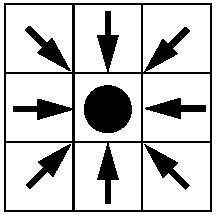
\includegraphics[width=0.1\textwidth, valign=B]{figs/neighbour}
	\caption{The Game of Life. An example of a large grid at two different times (separated by 9 steps) is shown in the left and middle panels. Here live cells are in black, dead are white. The evolution of the grid is governed by the birth and death of cells, where a cell's state is defined by its 8 neighbouring cells (right panel).}
	\label{fig:gol}
\end{figure}
\par 
The rules for evolving a system to the next time level are as follows:
\begin{itemize}
	\item {\color{ForestGreen}new cell born} if the cell has exactly three live neighbours - \textbf{\color{ForestGreen} ready to breed}.
	\item {\color{CornflowerBlue}state of cell unchanged} if the cell has exactly two live neighbours - \textbf{\color{CornflowerBlue}content}.
	\item {\color{Red}dies or stays dead} if the cell has $<2$ live neighbours - \textbf{\color{Red}lonely}.
	\item {\color{Red}dies or stays dead} if the cell has $>3$ live neighbours - \textbf{\color{Red}overcrowding}.
\end{itemize}

\par 
These rules are set so as to generate an equilibrium between living and dead cells. One can explore how altering the rules can affect the evolution of the system. To lax a {\color{ForestGreen} ready to bread} rule coupled with large amounts of {\color{Red}overcrowding allowed} can give rise to grids that quickly fill up with cells only to collapse entirely. 

\subsection{The ``Life'' in GOL} 
Using this fairly simple set of rules, some fairly complex structures can emerge\footnote{a nice list of types of structures is found on \href{https://en.wikipedia.org/wiki/Conway\%27s_Game_of_Life}{Wikipedia}}. The game is in fact Turing complete and can simulate a universal constructor or any other Turing machine. We highlight some common structures found in a typical game in Fig.\ref{fig:gol-structures}.

\begin{figure}[!h]	
	\centering
	
\includegraphics[height=0.06\textwidth, valign=c]{figs/Game_of_life_loaf.png}
	
\includegraphics[height=0.17\textwidth, valign=c]{figs/Game_of_life_pulsar.png}
	
\includegraphics[height=0.06\textwidth, valign=c]{figs/Game_of_life_animated_glider.png}
    
\includegraphics[height=0.11\textwidth, valign=c]{figs/Game_of_life_glider_gun.svg.png}
	\caption{Structures in GOL: We show an example of still life (left); oscillating life (middle); travelling life, so-called spaceships (right); and a constructor that generates gilder spaceships (bottom).}
	\label{fig:gol-structures}
\end{figure}

GOL may appear chaotic and can remain chaotic for long periods of time (even indefinitely) before settling into a combination of still lifes, oscillators, and spaceships. GOL is in fact undecidable, that is given an initial pattern and a later pattern, no algorithm exists that can tell whether the later pattern is ever going to appear using this IC. This is a corollary of the halting problem: the problem of determining whether a given program will finish running or continue to run forever from an initial input. 
\par 
The undecidability of the game depends on the rules and the dimensionality of the grid. For instance, increasing the dimension from 2 to 3 means that the rule for equilibrium goes from 2 neighbours out of 8 to 2 out of 26. You can try exploring the impact rules have on the game using the provided code repository discussed in the following section. 

\subsection{Grid-based simulations}
\label{sec:gol:gridsims}
At a basic level, \textbf{GOL} is a simulation of the temporal evolution of a 2-D grid. The rules governing the "life" can be arbitrarily complex and the grid need not be just two dimensional. If one changes a cell from just being alive or dead to having a complex internal state, increases the complexity of the rules and adds one more dimension,  \textit{you would have gone from GOL to any number of grid-based codes that are used to model physical processes}. This simple grid-based program should be viewed as the first step in writing more complex grid-based codes. 

\par 
As an example, ENZO (\cite{enzo}, repository is located \href{https://github.com/enzo-project/enzo-dev}{here}) is a Adaptive Mesh Refinement (AMR) code using Cartesian coordinates which can be run in one, two, and three dimensions, and supports a wide variety of physics including hydrodynamics, ideal and non-ideal magnetohydrodynamics. GOL would be equivalent to running ENZO in two dimensions where the "fluid" moves on the 2-D surface based on highly simplified equations. 

\section{Code Repository}\label{sec:code}
The code that forms the basis of the assignment is found on the course website. This repository contains the following 
\begin{itemize}
	\item basic files like a README, License
	\item \texttt{Makefile} setup to compile codes with a variety of different flags and features. For a quick tutorial on GNU Make, see \href{https://www.gnu.org/software/make/}{here}. Students are expected to be familiar with Make and the associated commands. Please familiarise yourself with this material. 
	\item Source code in \texttt{src/*c} (\texttt{C/C++}) and \texttt{src/*f90} (\texttt{Fortran}). We expect students to be familiar with \texttt{C/C++} and/or \texttt{Fortran}. All the source code provided is written in \texttt{C} and \texttt{Fortran}. Fortran source codes are noted by having \texttt{\_fort.f90} endings. Please feel free to change the make file to use a \texttt{C++} compiler when compiling the c codes and use C++ syntax if you so desire. 
	\item documentation and \LaTeX\ source code in \texttt{docs}
	\item a script to produce movies from png files when visualising with the PNG library. 
\end{itemize}
To familiarise yourself with the contents you can see what make options are available and browse the source directory. 
\begin{center}
\begin{minipage}{0.95\textwidth}
\small
\begin{minted}[frame=single,]{sh}
make allinfo # provides all the information of the commands listed below  
make configinfo # provides the different options available 
make makecommands # what you can make by typing these commands
make buildinfo # current compilers used
\end{minted}
\end{minipage}
\end{center}
You'll note that the make file is setup to accept command line arguments that can set compiler families such as \texttt{GCC}, \texttt{CRAY} when you type \texttt{make configinfo}. Try the following
\begin{center}
\begin{minipage}{0.95\textwidth}
\small
\begin{minted}[frame=single,]{sh}
# use the GNU CC family of compilers, gcc, g++, & gfortran AND 
# compile the serial version of the code, both C and Fortran sources.
make COMPILERTYPE=GCC cpu_serial 
# use the intel family of compilers and compile the openmp source codes (if present)
make COMPILERTYPE=INTEL cpu_openmp 
# use Cray compilers (useful for systems like magnus) and just compile the C sources 
make COMPILERTYPE=CRAY cpu_openmp_cc 
\end{minted}
\end{minipage}
\end{center}
Note that the code does require recent compilers so on machines such as zeus make sure to load a recent gcc compiler using commands such as \texttt{module swap gcc gcc/8.3.0})


\subsection{Source}
The common function calls with interface is provided in \texttt{src/common.*}, provide functions like visualising GOL, getting timing information, etc. We recommend students have a look at the prototypes in \texttt{src/common.h}. The key functions are:
\begin{center}
\begin{minipage}{0.95\textwidth}
\small
\begin{minted}[frame=single,]{c}
/// visualise the game of life
void visualise(enum VisualiseType ivisualisechoice, int step, int *grid, int n, int m);
/// generate IC
void generate_IC(enum ICType ic_choice, int *grid, int n, int m);
/// UI
void getinput(int argc, char **argv, struct Options *opt);
///GOL stats protoype
void game_of_life_stats(struct Options *opt, int steps, int *current_grid);
/// GOL prototype
void game_of_life(struct Options *opt, int *current_grid, int *next_grid, int n, int m);
\end{minted}
\end{minipage}
\end{center}
The \texttt{Fortran} source of \texttt{src/common\_fort.f90} provides a module with the same set of interfaces and subroutines. 
\begin{center}
\begin{minipage}{0.95\textwidth}
\small
\begin{minted}[frame=single,]{fortran}
module gol_common
    !   ascii visualisation
    subroutine visualise_ascii(step, grid, n, m)
    ! png visualisation
    subroutine visualise_png(step, grid, n, m)
    ! no visualisation
    subroutine visualise_none()
    ! visualisation routine
    subroutine visualise(ivisualisechoice, step, grid, n, m)
    ! generate random IC
    subroutine generate_rand_IC(grid, n, m)
    ! generate IC
    subroutine generate_IC(ic_choice, grid, n, m)
    ! UI
    subroutine getinput(opt)
    ! get some basic timing info
    real*8 function init_time()
    ! get the elapsed time relative to start
    subroutine get_elapsed_time(start)
end module
\end{minted}
\end{minipage}
\end{center}


The main program consists of (here we just highlight the \texttt{C} source as the \texttt{Fortran} source is similar): 
\begin{center}
\begin{minipage}{0.95\textwidth}
\begin{minted}[frame=single,]{c}
int main(int argc, char **argv)
{
    struct Options *opt = (struct Options *) malloc(sizeof(struct Options));
    getinput(argc, argv, opt);
    // allocate some memory 
    ... 
    // generate initial conditions 
    generate_IC(opt->iictype, grid, n, m);
    // start GOL while loopt 
    while(current_step != opt->nsteps){
        visualise(opt->ivisualisetype, current_step, grid, n, m);
        game_of_life_stats(opt, current_step, grid);
        game_of_life(opt, grid, updated_grid, n, m);
        // swap current and updated grid
        tmp = grid;
        grid = updated_grid;
        updated_grid = tmp;
        current_step++;
    }
    // free mem
    ...
}
\end{minted}
\begin{comment}
\begin{minted}{fortran}
! Fortran code 
program GameOfLife
    use gol_common 
    implicit none
    ... 
    ! get input 
    call getinput(opt)
    ! allocate some mem
    ...
    ! generate IC
    call generate_IC(opt%iictype, grid, n, m)
    do while (current_step .ne. nsteps)
        call visualise(opt%ivisualisetype, current_step, grid, n, m);
        call game_of_life_stats(opt, current_step, grid);
        call game_of_life(opt, grid, updated_grid, n, m);
        ! update current grid
        grid(:,:) = updated_grid(:,:)
        current_step = current_step + 1
    end do 
    ! deallocate mem 
    ..
end program GameOfLife
\end{minted}
\end{comment}
\end{minipage}
\end{center}
Implementations of the {\color{blue}\texttt{game\_of\_life}} and {\color{blue}\texttt{game\_of\_life\_stats}} functions can be found in \texttt{src/01\_cpu\_serial.c} (\& \texttt{src/01\_cpu\_serial\_fort.f90}). Familiarise yourself with these functions (based on your language of choice).  

\par 
Running the code is relatively simple.  
\begin{center}
\begin{minipage}{0.95\textwidth}
\small
\begin{minted}[frame=single,]{sh}
make cpu_serial
./bin/01_cpu_serial 
"Usage: ./bin/01_gol_cpu_serial <grid height> <grid width> "
  "[<nsteps> <IC type> <Visualisation type> <Rule type> <Neighbour type>"
  "<Boundary type> <stats filename>]"
./bin/01_cpu_serial 500 500 4 # run a 500x500 grid for 4 steps giving 
\end{minted}
	\fbox{\includegraphics[width=0.2\textwidth, valign=c]{figs/GOL.grid-500-by-500.step-0000.png}}
	\fbox{\includegraphics[width=0.2\textwidth, valign=c]{figs/GOL.grid-500-by-500.step-0001.png}}
	\fbox{\includegraphics[width=0.2\textwidth, valign=c]{figs/GOL.grid-500-by-500.step-0002.png}}
	\fbox{\includegraphics[width=0.2\textwidth, valign=c]{figs/GOL.grid-500-by-500.step-0003.png}}
\\	PNG Visualisation of output from GOL. FIlled black squares are living cells.
\end{minipage}
\end{center}

\subsection{Compiling on Pawsey systems}
The serial c and fortran codes will compile with all compilers on \texttt{magnus} so long as the appropriate compiler for the given programming environment is chosen. The make commands to use are 
\begin{itemize}
    \setlength{\itemindent}{70pt}
    \item[\texttt{PrgEnv-cray}:\quad]{\texttt{make COMPILERTYPE=CRAY}}
    \item[\texttt{PrgEnv-gnu}:\quad]{\texttt{make COMPILERTYPE=CRAY-GNU}}
    \item[\texttt{PrgEnv-intel}:\quad]{\texttt{make COMPILERTYPE=CRAY-INTEL}}
\end{itemize}
On other machines that do not make use of the Cray compiler wrappers, it is just a matter of specifying the appropriate compiler such as \texttt{make COMPILERTYPE=GNU} for \texttt{gnu} compilers.

\subsection{Expanded Rules}
Although not required for the assignment, you can alter the rules of the game, changing the number of neighbours that decide certain states, even expand the number of neighbours used and change the boundary conditions. A sample of the serial code structured to easily alter the rules for the game is \texttt{src/01\_gol\_serial\_expanded.c}.

\par 
This particular version of the code is an excellent start point for implementing far more complex rules, such as those governing the flow of a fluid or the diffusion of a gas across a surface.  


\newpage
\section{Assessable Tasks}\label{sec:tasks}
\subsection*{How to start?\nopunct\\} \label{sec:tasks:staring}
For each task, start by profiling the code using \texttt{gprof}. This will allow you to identify where most of the time is spent. Try using large grid sizes (within reason). With this profiling information, you should be able to identify what should be parallelised. Look at the code itself and make sure you understand the algorithm.

Copy the original serial source file to \texttt{02\_cpu\_openmp\_loop} and \texttt{02\_cpu\_openmp\_task} and try compiling the code
\begin{center}
\begin{minipage}{0.95\textwidth}
\begin{minted}[frame=single,]{sh}
# for C
cp src/01_cpu_serial.c src/02_cpu_openmp_loop.c
cp src/01_cpu_serial.c src/02_cpu_openmp_task.c
make cpu_openmp_cc
# for Fortran
cp src/01_cpu_serial_fort.f90 src/02_cpu_openmp_loop_fort.f90
cp src/01_cpu_serial_fort.f90 src/02_cpu_openmp_task_fort.f90
make cpu_openmp_fort
\end{minted}
\end{minipage}
\end{center}
Profile the code (for zeus, where we make sure to load a recent gcc compiler with \texttt{module swap gcc gcc/8.3.0}).
Here the example is for building on magnus.
\begin{center}
\begin{minipage}{0.95\textwidth}
\begin{minted}[frame=single,]{sh}
# compile
make COMPILERTYPE=CRAY PROFILER=ON cpu_openmp_loop_cc
# run two steps of a moderately large 100x100 grid
./bin/02_cpu_openmp_loop 100 100 2
# profile
gprof -lbp ./bin/02_cpu_openmp_loop gmon.out > analysis.txt
\end{minted}
\end{minipage}
\end{center}
Look at the output produced by the code as well as the output of the profiling.

The code provides summary statistics per step that depend only on the grid size and the step, saved as {\color{blue}\texttt{GOL-stats.txt}}. The code also writes to standard out, so when running save the output to meaningful log files. Similarly save the stats file to a meaning filename
\begin{center}
\begin{minipage}{0.95\textwidth}
\begin{minted}[frame=single,]{sh}
# lets set some variables for a run. Here numbers are examples only.
nomp=2
nxgrid=100
nygrid=100
nsteps=2
# set some meaningful name. Could be reference, latests, etc.
someversionname=reference
# set a base name
basename=GOL-${someversionname}.nomp-${nomp}.ngrid-${nxgrid}x${nygrid}.${nsteps}
export OMP_NUM_THREADS=${nomp}
./bin/02_cpu_openmp_loop ${nxgrid} ${nygrid} ${nsteps} > ${basename}.log
mv GOL-stats.txt ${basename}.stats.txt
\end{minted}
\end{minipage}
\end{center}
In this way, you can compare results as you update the code, change the number of threads, change versions, etc and keep track of changes in performance and compare results.

\subsection{{\color{Red} Preliminaries}: Correct Loop Ordering\nopunct\\}\label{sec:tasks:loop}
Both the C and Fortran codes do not have optimal do/for loops for the game of life grid. Please look at the code and update these loops to reduce cache misses (revisit material on serial optimisation if you are unclear about cache misses). Show that there is an improvement in the performance.

\subsection{{\color{Red} Principle Task}: Implement OpenMP Parallelism\nopunct\\}\label{sec:tasks:omp}
Perform an OpenMP parallelisation of the serial code, test performance and scaling. There are two main approaches, {\color{Orange}\textbf{Loop}} and {\color{Orange}\textbf{Task}} parallelism. This source code should be called \texttt{02\_cpu\_openmp\_loop.c} or \texttt{02\_cpu\_openmp\_loop\_fort.f90} (if using fortran) or for task parallelism or \texttt{02\_cpu\_openmp\_task.c} or \texttt{02\_cpu\_openmp\_task\_fort.f90} (if using fortran).

The code should contain extensive \textbf{\textit{comments}}, noting what you are doing \textit{and why}. I will compile your code using the appropriate \texttt{make} command.
{\centering \textit{You must show that the code produces correct results regardless of the number of OpenMP threads used. This can be checked with visualisation and also summary statistics.}}

\subsection{{\color{Red}Secondary Task}: Scaling Tests\nopunct\\}\label{sec:tasks:scaling}
Test how the code scales with number of threads and also problem size and discuss the observed behaviour. Start with 10x10 and increase the problem to 10000x10000 (or larger if you have the available memory). Increase the number of OpenMP threads from 1 to 16 (taking note of the number of actual logical cores on the system). Note that visualising each step significantly impacts the speed of the program, so we suggest running with visualisation turned off (that is provide an extra argument of \texttt{0 -1} so that the IC is the standard random IC but no visualisation is done.
\begin{center}
\begin{minipage}{0.95\textwidth}
\begin{minted}[frame=single,]{sh}
./bin/02_cpu_openmp_loop ${nxgrid} ${nygrid} ${nsteps} 0 -1
\end{minted}
\end{minipage}
\end{center}
Compare your results and explain the scaling seen both with problem size and number of threads. Please keep in mind that when running the scaling tests, submit sbatch jobs requesting exclusive access to a node on zeus by requesting all the resources and perform several tests.

\section{{\color{Blue}What you need to hand in\nopunct\\}}\label{sec:handin}

You must submit a zip (or tar) file containing:
\begin{itemize}
\item Your code within the repository so that it can be easily compiled. Make it clear which type of OpenMP parallelisation you have implemented.
\item A pdf of your code so that I can read it and the comments associated with the changes you have made. Remember to be verbose!
\item A pdf report discussing the OpenMP parallelisation of the code. Details of what should be in the report are outlined below.
\end{itemize}

\subsection*{Report\nopunct\\}\label{sec:handin:report}
\noindent Your report should contain the following sections:
  \begin{enumerate}
  \item{\textbf{Intro} : Describe language chosen, compilers used, any additional compilation flags used such as optimisation. Describe choice of parallelism used (if applicable).} 
  \item{\textbf{Profiling} : Profile the code and discuss the results.}
  \item{\textbf{Correctness} : Show code compiles and still produces correct results compared to serial version. Ensure that all 
functionality of the code remains intact. If you wish, you can add functionality.}
  \item{\textbf{Implementation} : Describe and discuss implementation, all choices and any testing that has driven a choice.}
  \item{\textbf{Scalability} : Test how the code performs, show scaling of code and discuss results.}
  \item{\textbf{Code} : Highlight changes to code.}
\end{enumerate}

\subsection*{Marks\nopunct\\}\label{sec:handin:marks}
\noindent The assignment is marked out of \textbf{30}. The marks are awarded as follows:
\begin{itemize}
  \item{\textbf{Correctness} : The code must compile and produce the correct result. \textbf{Otherwise a factor of 1/2 will be applied to the total mark.}}
  \item{\textbf{Profiling} : Out of 2}
  \item{\textbf{Implementation} and \textbf{Code}: Out of 20}
  \item{\textbf{Scalability}: Out of 8}
\end{itemize}

\noindent{\color{CornflowerBlue}BONUS}: \textit{If Both Task and Loop are implemented, bonus marks will be awarded.}

  %\item {\color{CornflowerBlue}BONUS}: Discuss how does thread affinity affects performance.
  %\item {\color{CornflowerBlue}BONUS}: Show that the code is also vectorised and how this affects performance.

\bibliographystyle{plain}
\begin{thebibliography}{2}

\bibitem{gol}
Gardner, Martin (October 1970), \textbf{Mathematical Games - The Fantastic Combinations of John Conway's New Solitaire Game 'Life'}, Scientific American (223): 120–123. \href{doi:10.1038/scientificamerican1070-120}{doi:10.1038/scientificamerican1070-120}

\bibitem{gol-wiki}
\href{https://en.wikipedia.org/wiki/Conway\%27s_Game_of_Life}{https://en.wikipedia.org/wiki/Conway\%27s\_Game\_of\_Life} and references therein.

\bibitem{enzo} Bryan, G.~L., Norman, M.~L., O'Shea, B.~W., et al.\ 2014, \textit{Astrophysical Journal Supplementary Series}, 211, 19. doi:10.1088/0067-0049/211/2/19

\end{thebibliography}

\end{document}
